% \begin{figure*}[ht!]
% \centering
% 	\begin{subfigure}{0.48\textwidth}
%                 \centering
% 		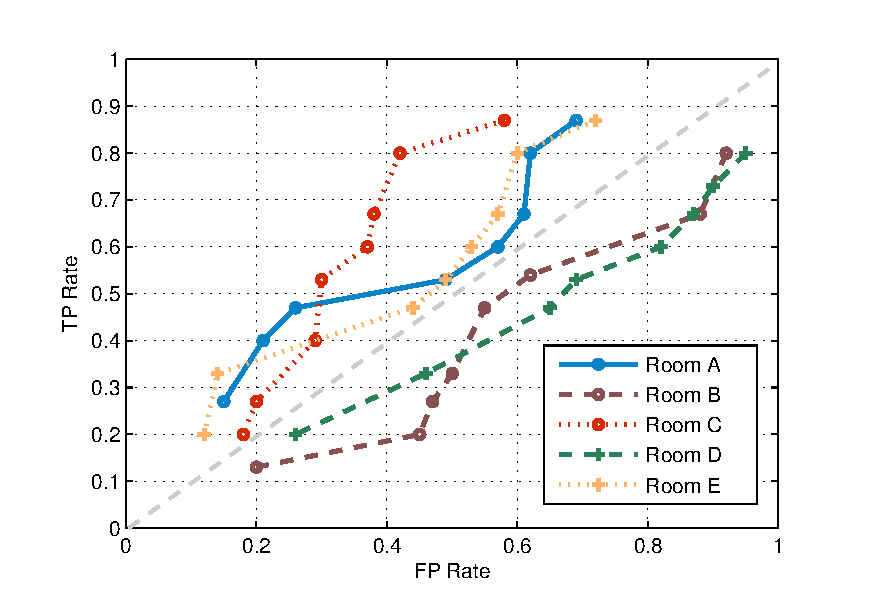
\includegraphics[width=\textwidth]{./fig/ROC_bsln.eps}
%                 \caption{Correlating the raw signals.}
% 	\end{subfigure}
% 	\begin{subfigure}{0.48\textwidth}
%                 \centering
% 		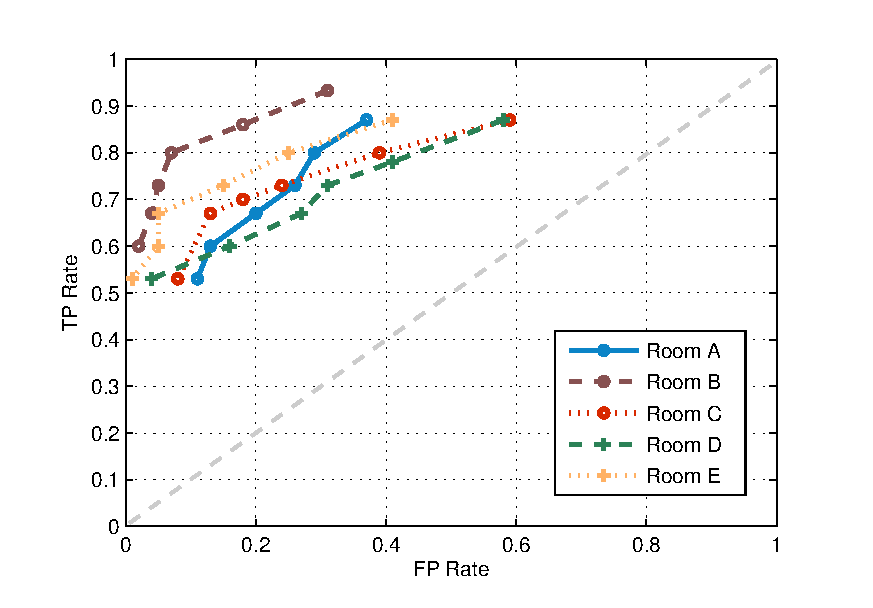
\includegraphics[width=\textwidth]{./fig/ROC_new.eps}
%                 \caption{Correlating the re-aggregated IMFs in the ``medium'' frequency band.}
%                 \label{fig:rocA}
% 	\end{subfigure}
% \caption{The ROC curves depict the sensitivity of the raw signal and mid-frequency IMFs to the threshold value. We choose the 0.2 FPR point as the boundary threshold for each room. }
% \label{fig:roc}
% \end{figure*}

\section{Evaluation}
To demonstrate the effectiveness as well as usefulness of methodology, we evaluate the technique in two different scenarios: a) intra building, that is, the training and testing data for classification is taken within the same building, and b) inter buildings, where training and testing resources are from two distinct buildings. We also show an application as a case study built based on the generated type information in two buildings, which would be impossible to achieve in the absence of categorical metadata. 

\subsection{Taxonamy}
In this paper, we consider 6 types of sensors, which are $CO_{2}$, humidity, room temperature, setpoint, air flow volume, other temperature. Specifically, room temperature includes only sensors that measure the air temperature of rooms and other temperatures covers all other temperature measurements such as supply air/return air/mixed air temperature and supply/return water temperature. We also put only one general type for setpoint which includes all types of setpoints instrumented in the buildings.

\subsection{Experimental Setup}
\begin{table}[ht!]
\caption{Number of Each Sensor Type}
\centering % used for centering table
\begin{tabular}{c c c}% centered columns (4 columns)
\hline %inserts single horizontal lines
Type & SDH & Rice \\ % inserts table 
%heading
\hline\hline % inserts double horizontal line
$CO_{2}$ & 1 & 2 \\ % inserting body of the table
humidity & 2 & 4 \\
room temp. & 3 & 2 \\
setpoint & 4 & 7 \\
air volume & 5 & 5 \\ % [1ex] adds vertical space
other temp. & 6 & 5 \\ % [1ex] adds vertical space
\hline %inserts single line
\end{tabular}
\label{table:roomspec} % is used to refer this table in the text
\end{table}

\subsection{Baseline and Metrics}
% We exploit a simple approach as baseline to compare with our proposed approach: instead of computing the correlation coefficients between re-aggregated IMFs of sensor feeds, we directly use the raw sensor data to do the correlation analysis and generate the two distributions for thresholding approach evaluation similarly to what described previously.

% As a baseline, we perform correlation analysis on the raw data. We generate two distributions, as previously described, and observe the effects of the choice of threshold on the true/false positive rate.
As a baseline, after we generate the two distributions described previously, we apply multidimensional scaling (MDS) to the corrcoeff matrix, in order to transform the original high-dimensional relative space to a 3-D space with an absolute origin, and run the k-means clustering algorithm.
We choose the true-positive rate (TPR, also known as recall rate) and false-positive rate (FPR) as metrics to evaluate the performance of our method versus the naive approach, which correlates the raw traces. A true-positive (TP) is when a sensor pair in a room is classified as being co-located 
while a false-positive (FP) is when a sensor that is not in room is classified as being so.
%is that a sensor not in room A is clustered as in room A.

\subsection{Intra Building Performance}

\subsection{Inter Building Performance}

% \begin{table}[h!]\footnotesize
%  \begin{center}
% 	\begin{tabular}{ r|c|c|c|c|c|c }
% 	\multicolumn{1}{r}{}
% 	 &  \multicolumn{1}{c}{$A$}
% 	 & \multicolumn{1}{c}{$B$}
% 	 & \multicolumn{1}{c}{$C$}
% 	 & \multicolumn{1}{c}{$D$}
% 	  & \multicolumn{1}{c}{$E$} \\
% 	\cline{2-6} 
% 	$SensorA_{1}$ & 1 & 0 & 0 & 0 & 0 & \checkmark\\
% 	\cline{2-6}
% 	$A_{2}$ & 1 & 0 & 0 & 0 & 0 & \checkmark\\
% 	\cline{2-6}
% 	$A_{3}$ & 1 & 0 & 0 & 0 & 0 & \checkmark\\
% 	\cline{2-6}
% 	$B_{1}$ & 0 & 1 & 0 & 0 & 0 & \checkmark\\
% 	\cline{2-6}
% 	$B_{2}$ & 0 & 1 & 0 & 0 & 0 & \checkmark\\
% 	\cline{2-6}
% 	$B_{3}$ & 0 & 1 & 0 & 0 & 0 & \checkmark\\
% 	\cline{2-6}
% 	$C_{1}$ & 0 & 0 & 1 & 0 & 0 & \checkmark\\
% 	\cline{2-6}
% 	$C_{2}$ & 0 & 0 & 1 & 0 & 0 & \checkmark\\
% 	\cline{2-6}
% 	$C_{3}$ & 0 & 0 & 1 & 0 & 0 & \checkmark\\
% 	\cline{2-6}
% 	$D_{1}$ & 0 & 0 & 0 & 1 & 0 & \checkmark\\
% 	\cline{2-6}
% 	$D_{2}$ & 0 & 0 & 0 & 1 & 0 & \checkmark\\
% 	\cline{2-6}
% 	$D_{3}$ & 0 & 0 & 1 & 0 & 0 & $\times$\\
% 	\cline{2-6}
% 	$E_{1}$ & 0 & 0 & 0 & 0 & 1 & \checkmark\\
% 	\cline{2-6}
% 	$E_{2}$ & 0 & 0 & 0 & 0 & 1 & \checkmark\\
% 	\cline{2-6}
% 	$E_{3}$ & 0 & 0 & 0 & 0 & 1 & \checkmark\\
% 	\cline{2-6}
% 	\end{tabular}
%  \end{center}
%  \caption{Clustering result using the thresholding method: a ``1" means the sensor is classified as inside the room. We get the ``\checkmark" and ``$\times$" by comparing the clustering results with ground truth.}
%  \label{tab:cluster}
% \end{table}

\subsection{Window Length Sensitivity and Training Bootstraping Analysis}

\subsection{Potential Misclassification}

\subsection{Case Study}
